\section{Western Blotting e Cromatografia di affinità}
Il \textbf{Western blotting} è una tecnica analitica che permette di rivelare, analizzare e quantificare le proteine. Questo metodo è utilizzato per rivelare molecole proteiche specifiche in campioni complessi.

Il Western blotting comporta tipicamente la separazione delle proteine mediante elettroforesi su gel seguita dal trasferimento su una membrana di nitrocellulosa.

Nel Western blotting le proteine vengono identificate mediante legami con anticorpi specifici. Generalmente si ricorre a una opportuna combinazione di un anticorpo primario e di un anticorpo secondario coniugato con HRP o AP per la rivelazione chemiluminescente o colorimetrica grazie all'impiego di un substrato appropriato. In alternativa, è possibile utilizzare un anticorpo primario o secondario con marcatura fluorescente per la visualizzazione diretta.

\subsection{Materiali e composti utilizzati}
\paragraph{Strumentazione}

\paragraph{Composti utilizzati}
\begingroup
\sisetup{
	propagate-math-font = true ,
	reset-math-version = false
}
\begin{itemize}
	\begin{multicols}{2}
		\itemb[Tampone di trasferimento]:
		\begin{itemize}[squareItem]
			\item \qty{20}{\milli\Molar} Tris
			\item \qty{152}{\milli\Molar} glicina
			\item \qty{20}{\percent} metanolo
		\end{itemize}
		\itemb[Soluzione di colorazione]:
		\begin{itemize}[squareItem]
			\item \qty{0.2}{\percent} Ponceau Red
			\item \qty{3}{\percent} \iupac{acido tricloroacetico}
		\end{itemize}
		\itemb[Tampone SBS \pH\ {\boldmath\num{7.2}} 10X]:
		\begin{itemize}[squareItem]
			\item \qty{1.37}{\g} \ch{NaCl}
			\item \qty{27}{\milli\Molar} \ch{KCl}
			\item \qty{15}{\milli\Molar} \ch{KH2PO4}
			\item \qty{81}{\milli\Molar} \ch{Na2HPO4}
		\end{itemize}
		\itemb[Soluzione di bloccaggio]:
		\begin{itemize}[squareItem]
			\item Tampone SBS \pH\ \num{7.2}
			\item \qty{0.2}{\percent} Tween
			\item \qty{5}{\percent} latte scremato in polvere
		\end{itemize}
		\itemb[Soluzione di sviluppo]:
		\begin{itemize}[squareItem]
			\item \qty{100}{\milli\Molar} Tris \ch{HCl} \pH\ \num{9.5}
			\item \qty{100}{\milli\Molar} \ch{NaCl}
			\item \qty{5}{\milli\Molar} \ch{MgCl2}\newline
			      \hspace*{-.5cm}Portare a \qty{10}{\ml} la soluzione e aggiungere:
			\item \qty{66}{\micro\litre} \gls{nbt}
			\item \qty{33}{\micro\litre} \gls{bcip}
		\end{itemize}
	\end{multicols}
\end{itemize}
\endgroup

\subsection{Protocollo}
\subsubsection{Western Blot}
\begin{enumerate}
	\item Al termine della corsa elettroforetica, sotto cappa chimica, immergere il gel nel tampone di trasferimento per \qty{30}{\sec}.
	\item All’interno del tampone di trasferimento, assemblare il sandwich:

	      \begin{minipage}[b]{0.35\textwidth}
		      \begin{itemize}[person]
			      \item Polo negativo
			      \item Spugna porosa
			      \item Carta da filtro
			      \item Gel
			      \item Nitrocellulosa
			      \item Carta da filtro
			      \item Spugna porosa
			      \item Polo positivo
		      \end{itemize}
	      \end{minipage}
	      \begin{minipage}[b]{0.6\textwidth}
		      \begin{figure}[H]
			      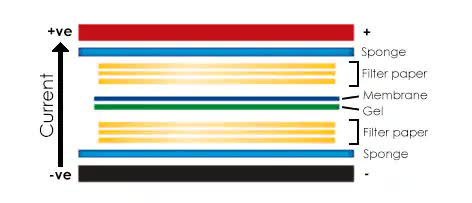
\includegraphics[scale=.5]{western-blot-diagram.jpeg}
		      \end{figure}
	      \end{minipage}

	\item Schiacciare con il mattarello per eliminare eventuali bolle d’aria
	\item Inserire il sandwich e il tampone di trasferimento in una vaschetta
	\item Applicare una differenza di potenziale
	\item Per verificare che il trasferimento sia avvenuto, colorare la membrana con il rosso di Ponceau.
	      \begin{Note}
		      La procedura è reversibile e non invasiva per permettere ulteriori test di carattere immunologico sul campione.
	      \end{Note}
	\item Lavare con acqua distillata per l'eccesso di colorante
	\item Segnare le bande con una matita
	\item Incubare la membrana nella soluzione di bloccaggio per \qty{1}{\hour} a temperatura ambiente, in agitazione. Questo procedimento è effettuato per saturare eventuali siti aspecifici della nitrocellulosa.

	      % Nota: la soluzione di bloccaggio è una soluzione proteica contenente latte in polvere a pH 7.2

	\item Incubare per \qty{1}{\hour} o più a temperatura in agitazione con anticorpo primario diluito nella soluzione di bloccaggio
	\item Lavare con la soluzione di bloccaggio 3 volte per \qty{5}{\min}, a temperatura ambiente, in agitazione. Procedimento effettuato per rimuovere eventuali anticorpi non legati
	\item Incubare per circa \qty{1}{\hour} a temperatura ambiente, con l’anticorpo secondario coniugato con la fosfatasi alcalina.
	\item Lavare 2 volte con la soluzione di bloccaggio per \qty{5}{\min} a temperatura ambiente
	\item Lavare con \qty{10}{\ml} di soluzione contenente \qty{1}{\ml} di tampone PBS diluito in acqua distillata
	\item Incubare il filtro nella soluzione di sviluppo. Composizione soluzione di sviluppo:
	      \begin{itemize}[person]
		      \item \qty{1.3}{\ml} di soluzione di sviluppo
		      \item Acqua fino al raggiungimento di \qty{10}{\ml} di volume
		      \item \qty{66}{\micro\litre} di NBT
		      \item \qty{33}{\micro\litre} di BCIP
	      \end{itemize}
	\item Quando la colorazione ha raggiunto un buon contrasto si blocca la reazione con \ch{H2O}
\end{enumerate}

\subsubsection{Cromatografia di affinità}
\begin{Informazione}
	La \textbf{cromatografia di affinità} è una tecnica cromatografica che si basa sulle interazioni che si formano tra una sostanza ed il relativo ligando.

	\vspace*{.3cm}
	Il processo è schematizzabile in tre fasi:
	\begin{enumerate}[person]
		\item aggiunta della miscela contenente l'analita con formazione del legame tra ligando e composto in esame
		\item si effettua la pulizia aggiungendo una opportuna soluzione di lavaggio che allontana le altre molecole presenti
		\item consiste nella scissione del legame con il ligando ad opera dell'eluente, che permette di separare la sostanza interessata portandola in soluzione
	\end{enumerate}
\end{Informazione}

\begin{enumerate}
	\item Aggiungere circa \qty{0.5}{\cm} di resina all’interno della colonna.
	      \begin{Note}
		      La resina è conservata in etanolo \qty{20}{\percent} perchè
	      \end{Note}
	\item Attendere la decantazione
	\item Aggiungere \qty{1}{\ml} di nichel.
	      \begin{Note}
		      Il nichel ha compito di consentire il legame tra il polimero e il tag di 6 istidine nelle proteine
	      \end{Note}
	\item Lavare per 3 volte con \qty{1}{\ml} di acqua distillata per eliminare i residui di etanolo.
	\item Equilibrare la colonna con \qty{1}{ml} di tampone Tris \qty{20}{\milli\Molar} \pH\ \num{8}
	\item Caricare \qty{500}{\ml} di campione GFP
	\item Recuperare il filtrato e ricaricarlo nella colonna
	\item Lavare 2 volte con \qty{750}{\micro\litre} di tampone Tris \qty{20}{\milli\Molar} \pH\ \num{8} recuperando il filtrato. Il filtrato viene recuperato per confrontare la luminescenza con quella dell’estratto finale.
	\item Preparare l’eluizione con \qty{1}{\ml} di tampone Tris \qty{20}{\milli\Molar} \pH\ \num{8} e \qty{50}{\micro\litre} di imidazolo
	\item Lavare la colonna con \qty{500}{\micro\litre} di eluizione. Ripetere il passaggio per due volte.
	\item Analizzare i campioni con luce blu e con spettrofotometro
\end{enumerate}

\begin{minipage}{0.3\linewidth}
	\img{11-01}{\\Menbrana dopo il trasferimento}{11-01}{trim={10cm 10cm 10cm 10cm},clip}
\end{minipage}
\hspace{0.35cm}
\begin{minipage}{0.3\linewidth}
	\img{11-02}{\\Campioni alla luce blu}{11-02}{}
\end{minipage}